\part{教程和指南}

\chapter{教程:为Karl学生作的一幅图}
本教程是写给PGF和TikZ的初学者的,因此不能够详尽考虑TikZ或者PGF的所有特征,只有一些你立刻会使用特征。

Karl是高中的数学和化学教师。他使用\LaTeX
的\tikzenv{picture}环境在他的工作活页和试卷中创建图形。
虽然图形的结果是可以接受的,但作图过程却非常冗长而繁琐。并且线的角度倾向有细微的错误,圆也不是很正常。当然,
他的学生不会注意直线是否是正确的角度,并且他们发现Kral的试题太难了,无论如何也不能够完美的把图画下来。但Karl
并不满足于现在的结果。

Karl的儿子也不太满意这样的结果(毕竟,他不用做这样的练习)。他告诉Karl希望用新的宏包来创建图形。有点混淆,
这个宏包似乎有两个名称:首先,Karl必须下载并安装PGF宏包。而结果在宏包中却是另一个被 称作TikZ的宏包,那是
一个支持标准 “TikZ ist kein Zeichenprogramm”的宏包。Karl认为这一切很奇怪,并且Tikz似乎并不做他所需
要的那些。尽管已经使用GUN软件很长一段时间了,但是有希望的。他的儿子向他保证TikZ的名字是用来警示人们TikZ不
是一个可以用鼠标或者平板电脑来绘制图形的程序,而更像一个“图形语言”。
\section{问题陈述}
Karl想在下一个工作活页上为学生画一幅图。他当前正在教授学生sin函数和cos函数。他想要得到如下图形:

\noindent
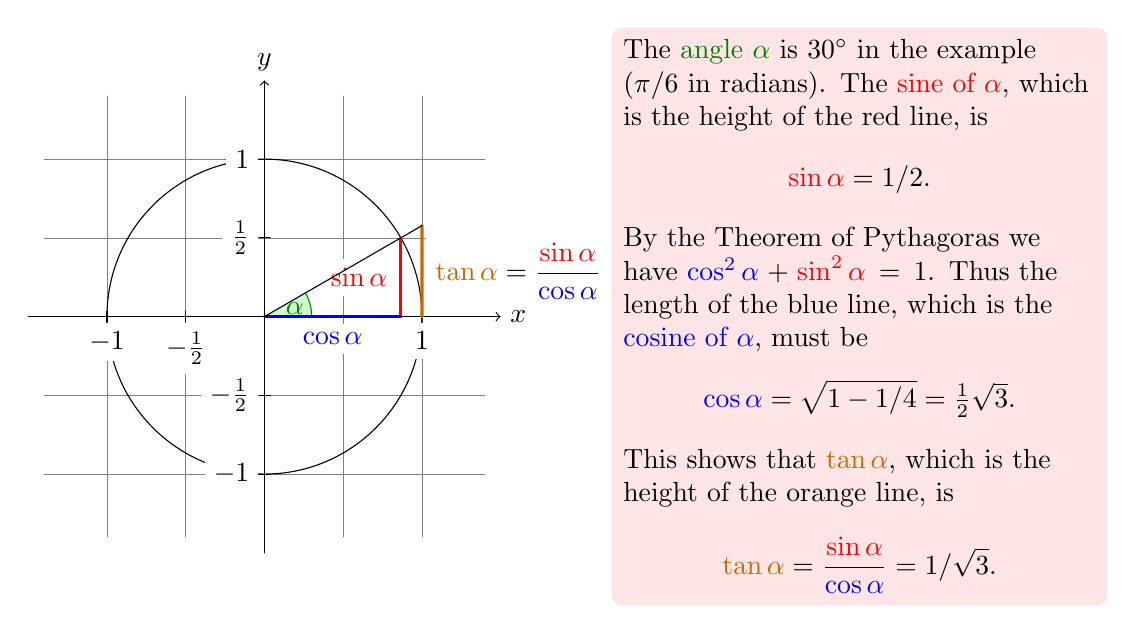
\begin{tikzpicture}
  [scale=2,line cap=round,
   % Styles
   axes/.style=,
   important line/.style={very thick},
   information text/.style={rounded corners,fill=red!10,inner sep=1ex}]

  % Local definitions
  \def\costhirty{0.8660256}

  % Colors
  \colorlet{anglecolor}{green!50!black}
  \colorlet{sincolor}{red}
  \colorlet{tancolor}{orange!80!black}
  \colorlet{coscolor}{blue}

  % The graphic
  \draw[help lines,step=0.5cm] (-1.4,-1.4) grid (1.4,1.4);

  \draw (0,0) circle (1cm);

  \begin{scope}[axes]
    \draw[->] (-1.5,0) -- (1.5,0) node[right] {$x$};
    \draw[->] (0,-1.5) -- (0,1.5) node[above] {$y$};

    \foreach \x/\xtext in {-1, -.5/-\frac{1}{2}, 1}
      \draw[xshift=\x cm] (0pt,1pt) -- (0pt,-1pt) node[below,fill=white] {$\xtext$};

    \foreach \y/\ytext in {-1, -.5/-\frac{1}{2}, .5/\frac{1}{2}, 1}
      \draw[yshift=\y cm] (1pt,0pt) -- (-1pt,0pt) node[left,fill=white] {$\ytext$};
  \end{scope}

  \filldraw[fill=green!20,draw=anglecolor] (0,0) -- (3mm,0pt) arc(0:30:3mm);
  \draw (15:2mm) node[anglecolor] {$\alpha$};

  \draw[important line,sincolor]
    (30:1cm) -- node[left=1pt,fill=white] {$\sin \alpha$} +(0,-.5);

  \draw[important line,coscolor]
    (0,0) -- node[below=2pt,fill=white] {$\cos \alpha$} (\costhirty,0);

  \draw[important line,tancolor] (1,0) --
    node [right=1pt,fill=white]
    {
      $\displaystyle \tan \alpha \color{black}=
      \frac{{\color{sincolor}\sin \alpha}}{\color{coscolor}\cos \alpha}$
    } (intersection of 0,0--30:1cm and 1,0--1,1) coordinate (t);

  \draw (0,0) -- (t);

  \draw[xshift=2.2cm] node [right,text width=6cm,information text]
    {
      The {\color{anglecolor} angle $\alpha$} is $30^\circ$ in the
      example ($\pi/6$ in radians). The {\color{sincolor}sine of
        $\alpha$}, which is the height of the red line, is
      \[
      {\color{sincolor} \sin \alpha} = 1/2.
      \]
      By the Theorem of Pythagoras we have ${\color{coscolor}\cos^2 \alpha} +
      {\color{sincolor}\sin^2\alpha} =1$. Thus the length of the blue
      line, which is the {\color{coscolor}cosine of $\alpha$}, must be
      \[
      {\color{coscolor}\cos\alpha} = \sqrt{1 - 1/4} = \textstyle
      \frac{1}{2} \sqrt 3.
      \]%
      This shows that {\color{tancolor}$\tan \alpha$}, which is the
      height of the orange line, is
      \[
      {\color{tancolor}\tan\alpha} = \frac{{\color{sincolor}\sin
          \alpha}}{\color{coscolor}\cos \alpha} = 1/\sqrt 3.
      \]%
    };
\end{tikzpicture}
\indent
\section{环境设置}
在TikZ中,为了画一幅图,首先需要告诉\TeX 或者\LaTeX 你要开始画图了。在\LaTeX 中使用\tikzenv{tikzpicture} 
环境,在plain \TeX 中使用\tikzcom{tikzpicture} 来开始画图,用\tikzcom{endtikzpicture} 来结束绘图。
\subsection{\LaTeX 环境设置}
Karl是\LaTeX 用户,因此设置他的文件如下:

\begin{lstlisting}
\documentclass{article}% say
\usepackage{tikz}
\begin{document}
We are working on 
\begin{tikzpicture}
  \draw(-1.5,0)--(1.5,0);
  \draw(0,-1.5)--(0,1.5); 
\end{tikzpicture}
\end{document}
\end{lstlisting}
通过执行pdflatex或者latex之后执行dvips,将产生像下图所示的结果:

\noindent
we are working on 
\begin{tikzpicture}[information text/.style={rounded corners,fill=red!10,inner sep=1ex}]
\draw(-1.5,0)--(1.5,0);
\draw(0,-1.5)--(0,1.5);
\draw[xshift=2.2cm] node[right,text width=6cm,information text]
{
we are working on
\begin{lstlisting}
\begin{tikzpicture}
\draw(-1.5,0)--(1.5,0);
\draw(0,-1.5)--(0,1.5);
\end{tikzpicture}.
\end{lstlisting}
};
\end{tikzpicture}

\indent
不可否认,现在不是完整的图,但是我们已经建立了坐标轴。好吧,不完整,但我们用直线绘制出了坐标轴。Karl突然有了失落的感
觉,离他要绘制的图仍然有很大的距离。

让我们更仔细的看看代码。首先,tikz宏包被加载了,它被称作PGF基础系统的前台。在本手册中被描述的基础层是更加基础的、更难
以使用的。前台提供简单的语法来完成相同的事。

在环境中有两个\tikzcom{draw}命令。它们意味着:“要绘制的路径被随后的命令明确直到分号为止”。第一条路径被明确为
\lstinline$(-1.5,0)--(1.5,0)$,它意味着直线从位于\lstinline$(-1.5,0)$的点开始到位于\lstinline$(1.5,0)$的
点结束。在此,位置被明确为内部最初的1cm为一个单位的精确地坐标系统。

Karl十分高兴环境自动地保留足够的空间用于包含图形。

\subsection{Plain \TeX 环境设置}
碰巧Karl的妻子Gerda也是一位数学教师,她不是\LaTeX 用户,但她使用plain\TeX ,因为她喜欢用“老方式”做事情。她也能够
使用TikZ。她应当用\lstinline$\input$ tikz.tex替代\  \lstinline$\begin${tikzpicture},并用\ \tikzcom{tikzpicture}替\ 代\lstinline$\begin{tikzpicture}$,用\ \tikzcom{endtikzpicture}替代\ \lstinline$\end{tikzpicture}$。

因此,她会用:
\begin{lstlisting}
% % Plain TeX file
\input tikz.tex
\baselineskip=12pt
\hsize=6.3truein
\vsize=8.7truein
We are working on 
\tikzpicture
  \draw(-1.5,0)--(1.5,0);
  \draw(0,-1.5)--(0,1.5);
\endtikzpicture.
\bye
\end{lstlisting}

Gerda能够用pdfex或者tex与dvips一起实现对止述文件的排版。TikZ会自动识别她所使用的的驱动程序。如果她希望能够使用dvipdfm与
tex一起工作。她将需要修改pgf.cfg文件,或者在引入tikz.tex或者pgf.tex前加入\lstinline$\def\pgfsysdriver{pgfsys-dvipdfm.def}$。

\subsection{Con\TeX t 环境设置}
Karl的舅舅Hans使用Con\TeX t。像Gerda一样,Hans也可使用TikZ。他要用\ \lstinline$\usemodule$ [tikz]\ 替代\ \lstinline$\usepackage$ {tikz},用\tikzcom{starttikzpicture}替代\lstinline$\begin$ {tikzpicture},用\tikzcom{stoptikzpicture}替代\lstinline$\end{tikzpicture}$。

他的例子正如下面的那样:
\begin{lstlisting}
%% ConTeXt file
\usemodule[tikz]
\starttext
  We are working on 
   \strttikzpicture
    \draw(-1.5,0)--(1.5,0);
    \draw(0,-1.5)--(0,1.5);
   \stoptikzpicture.
 \stoptext
\end{lstlisting}

Hans用texexec进行该文件的排版。
\section{创建直线路径}

在TikZ中所有图片的基本构建块是路径。路径是构建的一系列的直线和曲线。通过在一对括号中明确起点位置的坐标来开始一条路径,接下来是
一系列的“路径延展操作”,最简单的是我们所使用过的--。其后面必须跟另外一个确切的坐标,并在直线上延展该路径至该新的坐标位置。例如,
如果我们将两条路径转换成来一条路径,将得到下面的结果:

\begin{tikzpicture}[information text/.style={rounded corners,fill=red!10,inner sep=1ex}]
\draw(-1.5,0)--(1.5,0)--(0,-1.5)--(0,1.5);
\draw[xshift=2cm] node[right,text width=10cm,information text]
{
\begin{lstlisting}
\tikz\draw(-1.5,0)--(1.5,0)--(0,-1.5)--(0,1.5);
\end{lstlisting}
};
\end{tikzpicture}

在此没有{tikzpicture}环境,Karl稍感困惑。反而,使用了短命令\tikzcom{tikz}。该命令带一个参数或者将随后直到分号为止的东西
收集起来放来{tikzpicture}环境中。一般来讲,所有的TikZ绘图命令必须出现在\lstinline$\tikz$的参数中,或者位置{tikzpicture}
环境中。幸运地是,\lstinline$\draw$命令仅仅被定义于环境之中,因此你将不会有任何犯错的机会。

\section{创建曲线}
接来,Karl想画圆。要画圆,直线显然是做不到的,需要某种方式来完成曲线的绘制。为此TikZ提供了一特殊的语法来完成曲线的绘制。它需要一到两个控制点。这背后的数学并不是很琐碎,但其基本思想是:假设你位于点$x$,并且第一个控制点是$y$。曲线将在$x$点沿着$y$的方向开始绘制。就是说,曲线的切线位于点$x$并指向点$y$。接下来,曲线将在点$z$结束,其控制点是$w$。曲线直接在点$z$处结束,并且它的切线位于点$z$并指向点$w$。

这里有一个示例(控制点已经清楚的注明):


\begin{tikzpicture}[information text/.style={rounded corners,fill=red!10,inner sep=1ex}]
\filldraw[gray](0,0)circle(2pt)
(1,1)circle(2pt)
(2,1)circle(2pt)
(2,0)circle(2pt);
\draw(0,0)..controls(1,1)and(2,1)..(2,0);
\draw[xshift=2.5cm] node[right,text width=11cm,information text]
{
	\begin{lstlisting}
	\begin{tikzpicture}
	\filldraw[gray] (0,0)circle(2pt)
	(1,1)circle(2pt)
	(2,1)circle(2pt)
	(2,0)circle(2pt);
	\draw(0,0)..controls(1,1)and(2,1)..(2,0);
	\end{tikzpicture}.
	\end{lstlisting}
};
\end{tikzpicture}


延展曲线的一般语法是“..controls$<$first control point$>$ and $<$second control point$>$..$<$end point$>$”。你可以省略and $<$second control point$>$,则第一个控制点将被使用两次。

因此,Karl可为他的图片画第一个半圆了:

\noindent
\begin{tikzpicture}[information text/.style={rounded corners,fill=red!10,inner sep=1ex}]
\draw(-1.5,0)--(1.5,0);
\draw(0,-1.5)--(0,1.5);
\draw(-1,0)..controls(-1,0.555)and(-0.555,1)..(0,1)..controls(0.555,1)and(1,0.555)..(1,0);
\draw[xshift=2cm] node[right,text width=11cm,information text]
{
\begin{lstlisting}
\begin{tikzpicture}
\draw(-1.5,0)--(1.5,0);
\draw(0,-1.5)--(0,1.5);
\draw(-1,0)..controls(-1,0.555)and(-0.555,1)..(0,1)	
..controls(0.555,1)and(1,0.555)..(1,0);
\end{tikzpicture}.
\end{lstlisting}
};
\end{tikzpicture}
\indent

Karl对这个结果非常满意,但是用这样的方式来描述一个圆是非常笨拙的。幸运的是还有更简单的方式来完成这个任务。

\section{创建圆}

要创建一个圆,可以使用路径创建操作circle\index{circle}来完成。该操作由后面括号中的数字来指定其半径,如下面的例子所示:

\begin{tikzpicture}[information text/.style={rounded corners,fill=red!10,inner sep=1ex}]
\draw(0,0)circle(10pt);
\draw[xshift=2cm] node[right,text width=11cm,information text]
{
	\begin{lstlisting}
	\tikz\draw(0,0)circle(10pt);
	\end{lstlisting}
};
\end{tikzpicture}
\indent

使用ellipse操作可以添加一个椭圆。需要指定两个方向的半径,一个是$x$方向,另一个是$y$方向,并用and进行分隔:

\begin{tikzpicture}[information text/.style={rounded corners,fill=red!10,inner sep=1ex}]
\draw(0,0)ellipse(20pt and 10pt);
\draw[xshift=2cm] node[right,text width=11cm,information text]
{
	\begin{lstlisting}
	\tikz\draw(0,0)ellipse(20pt and 10pt);
	\end{lstlisting}
};
\end{tikzpicture}
\indent
不仅可以画水平方向和垂直方向的椭圆,还能够绘制任意方向的椭圆。可以通过变换来实现,关于变换我们将在后面进行讲解。创建一个小椭圆的代码是\lstinline$\tikz \draw[rotate=30](0,0)ellipse(6pt and 3pt);$。

回到karl的问题,他可以写代码\lstinline$\draw(0,0)circle(1cm);$来画圆:

\noindent
\begin{tikzpicture}[information text/.style={rounded corners,fill=red!10,inner sep=1ex}]
\draw(-1.5,0)--(1.5,0);
\draw(0,-1.5)--(0,1.5);
\draw(0,0)circle(1cm);
\draw[xshift=2cm] node[right,text width=11cm,information text]
{
	\begin{lstlisting}
	\begin(tikzpicture)
	\draw(-1.5,0)--(1.5,0);
	\draw(0,-1.5)--(0,1.5);
	\draw(0,0)circle(1cm);
	\end{tikzpicture}
	\end{lstlisting}
};
\end{tikzpicture}
\indent

此时,karl有些担忧,这个是这么小,而他要完成的图比这个图要大很多。他很乐于学习TikZ,因为TikZ有很强的变换选项,并且通过三个因素能够很容易地的调节图形的尺寸。到目前为,我们使用小尺寸是为了节省空间。

\section{创建矩形}

接下来要生成背景中的栅格。通常有好几种方式可以用于栅格的生成。例如,可以画很多矩形。由于矩形比较通用,其语法是:要在当前路径中添加矩形,需要使用rectangle路径创建操作。该操作的后面接另一个坐标,并双师前一坐村和后一坐标为角点来添加矩形。好了,让我们在图中添加两个矩形:

\noindent
\begin{tikzpicture}[information text/.style={rounded corners,fill=red!10,inner sep=1ex}]
\draw(-1.5,0)--(1.5,0);
\draw(0,-1.5)--(0,1.5);
\draw(0,0)circle(1cm);
\draw(0,0)rectangle(0.5,0.5);
\draw(-0.5,-0.5)rectangle(-1,-1);
\draw[xshift=2cm] node[right,text width=11cm,information text]
{
	\begin{lstlisting}
	\begin(tikzpicture)
	\draw(-1.5,0)--(1.5,0);
	\draw(0,-1.5)--(0,1.5);
	\draw(0,0)circle(1cm);
	\draw(0,0)rectangle(0.5,0.5);
	\draw(-0.5,-0.5)rectangle(-1,-1);
	\end{tikzpicture}
	\end{lstlisting}
};
\end{tikzpicture}
\indent

然后,这也许更适合其它情况,却并不适合Karl的问题:首先,我们需要很多的矩形,而且它们的边界也不是“封闭的”。

因此,在知道grid操作前Karl打算凭借\lstinline$\draw$命令来给制四条水平线和垂直线来实现栅格。

\section{栅格创建}

grid路径操作用于在当前路径中创建栅格。该操作将添加一系列的直线用来构成栅格并填充到由当前点和grid操作之后的点所构成的矩形区域。例如代码:\lstinline$\tikz \draw[step=2pt] (0,0) grid (10pt,10pt);$产生\tikz \draw[step=2pt](0,0)grid(10pt,10pt);值得注意的是,\lstinline$\draw$的参数选项用于指定栅格的宽度(也可以用xstep和ystep定义各自的距离).随着Karl学习的深入,将会有更多类似有影响的选项。

对于Karl来说,代码可以这样写:

\noindent
\begin{tikzpicture}[information text/.style={rounded corners,fill=red!10,inner sep=1ex}]
\draw(-1.5,0)--(1.5,0);
\draw(0,-1.5)--(0,1.5);
\draw(0,0)circle(1cm);
\draw[step=.5cm](-1.4,-1.4)grid(1.4,1.4);
\draw[xshift=2cm] node[right,text width=11cm,information text]
{
	\begin{lstlisting}
	\begin(tikzpicture)
	\draw(-1.5,0)--(1.5,0);
	\draw(0,-1.5)--(0,1.5);
	\draw(0,0)circle(1cm);
	\draw[step=.5cm](-1.4,-1.4)grid(1.4,1.4);
	\end{tikzpicture}
	\end{lstlisting}
};
\end{tikzpicture}
\indent

再来看看需要的图片,Karl注意到使栅格变淡一点会更好一些(他的儿子告诉他,如果栅格不变淡的话,往往会使人注意力分散)。为了减淡栅格,Karl在\lstinline$\draw$命令中增加了更多的选项用于绘制栅格。首,他对栅格线的颜色设置为gray。其次,把线宽调整为very thin。 最后,他调整了命令的顺序,使栅格最先画,而其它的由绘于其上:

\noindent
\begin{tikzpicture}[information text/.style={rounded corners,fill=red!10,inner sep=1ex}]
\draw[step=.5cm,gray,very thin](-1.4,-1.4)grid(1.4,1.4);
\draw(-1.5,0)--(1.5,0);
\draw(0,-1.5)--(0,1.5);
\draw(0,0)circle(1cm);
\draw[xshift=2cm] node[right,text width=11cm,information text]
{
\begin{lstlisting}
\begin(tikzpicture)
\draw[step=.5cm,gray,very thin](-1.4,-1.4)
	grid(1.4,1.4);
\draw(-1.5,0)--(1.5,0);
\draw(0,-1.5)--(0,1.5);
\draw(0,0)circle(1cm);	
	\end{tikzpicture}
	\end{lstlisting}
};
\end{tikzpicture}
\indent
\endinput